\documentclass{article}

\def\ParSkip{} 
% Packages
\usepackage{amssymb,amsmath,amsthm,bbm}
\usepackage{verbatim,float,url,dsfont}
\usepackage{graphicx,subfigure,psfrag}
\usepackage{algorithm,algorithmic}
\usepackage{mathtools,enumitem}
\usepackage{multirow}
\usepackage{ragged2e}
\usepackage{xr-hyper}
\usepackage{array}

\usepackage[colorlinks=true,citecolor=blue,urlcolor=blue,linkcolor=blue]{hyperref}
\usepackage[margin=1in]{geometry}
\usepackage[round]{natbib}

\usepackage[utf8]{inputenc} % allow utf-8 input
\usepackage[T1]{fontenc}    % use 8-bit T1 fonts
\usepackage{booktabs}       % professional-quality tables
\usepackage{nicefrac}         % compact symbols for 1/2, etc.
\usepackage{microtype}      % microtypography

\ifdefined\TimesFont 
\usepackage{times} % use times font
\fi

\ifdefined\ParSkip 
\usepackage{parskip} % use par skip
\fi

% Theorems and such
\newtheorem{theorem}{Theorem}
\newtheorem{lemma}{Lemma}
\newtheorem{corollary}{Corollary}
\newtheorem{proposition}{Proposition}
\theoremstyle{definition}
\newtheorem{remark}{Remark}
\newtheorem{definition}{Definition}

% Assumption
\newtheorem*{assumption*}{\assumptionnumber}
\providecommand{\assumptionnumber}{}
\makeatletter
\newenvironment{assumption}[2]{
  \renewcommand{\assumptionnumber}{Assumption #1#2}
  \begin{assumption*}
  \protected@edef\@currentlabel{#1#2}}
{\end{assumption*}}
\makeatother

% Widebar
\makeatletter
\newcommand*\rel@kern[1]{\kern#1\dimexpr\macc@kerna}
\newcommand*\widebar[1]{%
  \begingroup
  \def\mathaccent##1##2{%
    \rel@kern{0.8}%
    \overline{\rel@kern{-0.8}\macc@nucleus\rel@kern{0.2}}%
    \rel@kern{-0.2}%
  }%
  \macc@depth\@ne
  \let\math@bgroup\@empty \let\math@egroup\macc@set@skewchar
  \mathsurround\z@ \frozen@everymath{\mathgroup\macc@group\relax}%
  \macc@set@skewchar\relax
  \let\mathaccentV\macc@nested@a
  \macc@nested@a\relax111{#1}%
  \endgroup
}
\makeatother

% Min and max
\newcommand{\argmin}{\mathop{\mathrm{argmin}}}
\newcommand{\argmax}{\mathop{\mathrm{argmax}}}
\newcommand{\minimize}{\mathop{\mathrm{minimize}}}
\newcommand{\maximize}{\mathop{\mathrm{maximize}}}
\newcommand{\st}{\mathop{\mathrm{subject\,\,to}}}

% Shortcuts
\def\R{\mathbb{R}}
\def\C{\mathbb{C}}
\def\Z{\mathbb{Z}}
\def\N{\mathbb{N}}
\def\E{\mathbb{E}}
\def\P{\mathbb{P}}
\def\T{\mathsf{T}}
\def\Cov{\mathrm{Cov}}
\def\Var{\mathrm{Var}}
\def\indep{\perp\!\!\!\perp}
\def\th{^{\text{th}}}
\def\tr{\mathrm{tr}}
\def\df{\mathrm{df}}
\def\dim{\mathrm{dim}}
\def\col{\mathrm{col}}
\def\row{\mathrm{row}}
\def\nul{\mathrm{null}}
\def\rank{\mathrm{rank}}
\def\nuli{\mathrm{nullity}}
\def\spa{\mathrm{span}}
\def\sign{\mathrm{sign}}
\def\supp{\mathrm{supp}}
\def\diag{\mathrm{diag}}
\def\aff{\mathrm{aff}}
\def\conv{\mathrm{conv}}
\def\dom{\mathrm{dom}}
\def\hy{\hat{y}}
\def\hf{\hat{f}}
\def\hmu{\hat{\mu}}
\def\halpha{\hat{\alpha}}
\def\hbeta{\hat{\beta}}
\def\htheta{\hat{\theta}}
\def\cA{\mathcal{A}}
\def\cB{\mathcal{B}}
\def\cD{\mathcal{D}}
\def\cE{\mathcal{E}}
\def\cF{\mathcal{F}}
\def\cG{\mathcal{G}}
\def\cK{\mathcal{K}}
\def\cH{\mathcal{H}}
\def\cI{\mathcal{I}}
\def\cL{\mathcal{L}}
\def\cM{\mathcal{M}}
\def\cN{\mathcal{N}}
\def\cP{\mathcal{P}}
\def\cS{\mathcal{S}}
\def\cT{\mathcal{T}}
\def\cW{\mathcal{W}}
\def\cX{\mathcal{X}}
\def\cY{\mathcal{Y}}
\def\cZ{\mathcal{Z}}

\DeclareMathOperator*{\esssup}{ess\,sup}

\title{Nonparametric Regression: Splines and RKHS Methods \\ \smallskip
\large Advanced Topics in Statistical Learning, Spring 2023 \\ \smallskip
Ryan Tibshirani}
\author{}
\date{}

\begin{document}
\maketitle
\RaggedRight
\vspace{-50pt}

Note: we're following the context, problem setup, notation, etc. from the last
lecture on nonparametric regression.

\section{Regression splines}

Regression splines and smoothing splines are motivated from a different
perspective than kernels and local polynomials; in the latter case, we started
off with a special kind of local averaging, and moved our way up to a
higher-order local models. With regression splines and smoothing splines, we
build up our estimate globally, from a set of select basis functions. 

(We note that, at a broader level, the latter is often called the
\emph{synthesis} framework for modeling, where we build up our estimate from a
set of atoms---here being basis functions.) 

\subsection{Splines}

These basis functions, as you might guess, are \emph{splines}. Let's assume that
$d=1$. We'll stick to the univariate case for a little while, because splines
are complex and interesting enough in dimension $d=1$. A spline $f$ of degree
$k$ with knots at $t_1 < \dots < t_r$ is a piecewise polynomial of degree $k$  
that is continuous and has continuous derivatives of orders $1,\dots,k-1$ at its
knots. To be clear: 
\begin{itemize}
\item $f$ is a polynomial of degree $k$ on each of $(-\infty,t_1], [t_1,t_2],
  \dots, [t_r,\infty)$; and
\item $D^\ell f$ is continuous at each of $t_1,\dots,t_r$, for all
  $\ell=0,\dots,k-1$. 
\end{itemize}

Splines have some special (some might say amazing) properties, and we will only
really scratch the surface here. They have been a topic of interest among
mathematicians and statisticians for a long time. Informally, a spline is a lot
smoother than a piecewise polynomial, and so modeling with splines can serve as
a way of reducing the variance of an estimator. See Figure \ref{fig:splines} for
an illustration.  

\begin{figure}[tb]
\centering
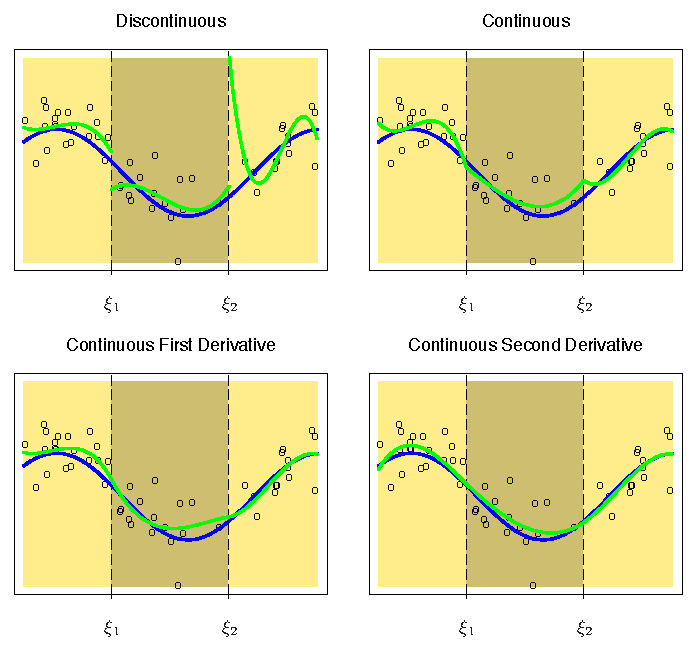
\includegraphics[width=0.8\textwidth]{splines.pdf}
\caption{\it Illustration of the effects of enforcing continuity at the knots
  for a cubic piecewise polynomial, and for various orders of the derivative,
  Credit: Chapter 5 of \citet{hastie2009elements}.}    
\label{fig:splines}
\end{figure}

A bit of statistical folklore: it is said that a cubic spline is so smooth, that
one cannot detect the locations of its knots by eye! 

\subsection{Spline bases}

How can we parametrize the space of $k\th$ degree splines with knots at 
$t_1,\dots,t_r$?  The most natural way is to use the \emph{truncated power
  basis}, $g_1, \dots, g_{r+k+1}$, defined as   
\begin{equation}
\begin{gathered}
\label{eq:tpb}
g_j(x) = \frac{1}{(j-1)!} x^j, \quad j=1,\dots,k+1, \\
g_{j+k+1}(x) = \frac{1}{k!} (x-t_j)^k_+, \quad j=1,\dots,r,
\end{gathered}
\end{equation}
Here $x_+=\max\{x,0\}$ denotes the positive part of $x$. From this we can see
that the linear space of $k\th$ degree splines with knots at $t_1,\dots,t_r$ has 
dimension $r+k+1$.

While \eqref{eq:tpb} gives us a simple and natural basis, calculations involving
truncated power bases functions can be troublesome because the ensuing basis 
matrix, $G \in \R^{n \times (r+k+1)}$ with entries
\[
G_{ij} = g_j(x_i)
\]
is generally very poorly conditioned.

A much better computational choice, both for speed and numerical stability, is 
called the \emph{B-spline basis}. This was a major development in spline theory 
and is now much the standard in software. The key idea is that B-splines have
local support: each B-spline basis function for a $k\th$ degree spline space is
supported on $k+2$ knots. Therefore the corresponding basis matrix is banded. It
also tends to be much better conditioned.  

Defining B-splines is certainly requires more nuance than the truncated power
basis, and the precise form of a B-spline is unimportant for the rest of this
lecture. For completeness, you can find the details behind their construction in
Appendix \ref{app:bs}. (You can also jump to Figure \ref{fig:bs} for a visual.) 

\subsection{Regress away!}

A first idea: let's just perform regression on a spline basis. In other words,
we use as our working model a $k\th$ degree spline with knots at some pre-fixed 
locations $t_1,\dots,t_r$. This means expressing $f$ as  
\[
f = \sum_{j=1}^{r+k+1} \beta_j g_j
\]
where $\beta_1,\dots,\beta_{r+k+1} \in \R$ are coefficients and
$g_1,\dots,g_{r+k+1}$ is a basis for the space of $k\th$ degree splines over the
knots $t_1,\dots,t_r$; for example, the truncated power basis or B-spline basis.    

Letting $Y=(y_1,\dots,y_n) \in \R^n$ denote the response vector, and defining
the basis matrix $G \in \R^{n \times (r+k+1)}$ as before, to have entries
\[
G_{ij} = g_j(x_i),
\]
we then just use least squares regression to determine estimate the
coefficients, defining \smash{$\hbeta = (\hbeta_1,\dots,\hbeta_{r+k+1})$} to
solve 
\[
\minimize_\beta \; \|Y - G\beta\|_2^2.
\]
This yields the \emph{regression spline} estimator, which makes predictions
according to   
\[
\hf(x) = \sum_{j=1}^{r+k+1} \hbeta_j g_j(x).
\]
Of course we know that \smash{$\hbeta = (G^\T G)^{-1} G^\T Y$}, so we can write
this as 
\[
\hf(x) = (g_1(x),\dots,g_{r+k+1}(x))^\T (G^\T G)^{-1} G^\T Y = w(x)^\T Y,  
\]
which reveals that regression splines are linear smoothers.

This is a classic method, and can work well provided that we choose ``good''
knots $t_1,\dots,t_r$; but in general choosing knots is a tricky business. There
is a large literature on knot selection for regression splines via greedy
methods like recursive partitioning. In practice, smoothing splines seem to be
more popular, which we cover next.

\section{Smoothing splines}

Before delving into smoothing splines, we need to introduce a variant on the
usual spline definition given above. To motivate it: a problem with spline
estimates is that they can have somewhat erractive behavior---translating into
high variance---at the boundaries of the input domain. (Recall that this is the
opposite problem to that with kernel smoothing, which had poor bias at the
boundaries.) This only gets worse as the polynomial order $k$ gets larger.   

\subsection{Natural splines}

One way to remedy this problem is to force the piecewise polynomial function to
have a lower degree to the left of the leftmost knot, and to the right of the
rightmost knot---this is exactly what \emph{natural splines} do. A natural
spline $f$ of degree $k$ with knots at $t_1 < \dots < t_r$ is a piecewise
polynomial of degree $k$ such that:
\begin{itemize}
\item $f$ is a polynomial of degree $k$ on each of $[t_1,t_2], \dots,
  [t_{r-1},t_r]$; 
\item $f$ is a polynomial of degree $(k-1)/2$ on $(-\infty,t_1]$ and
  $[t_r,\infty)$; and 
\item $D^\ell f$ is continuous at each of $t_1,\dots,t_r$, for all
  $\ell=0,\dots,k-1$. 
\end{itemize}
It is implicit here that natural splines are only defined for an odd degree $k$
(linear, cubic, etc.) The choice $k=3$ yields a natural cubic spline, by far the
most common case: this is just a cubic spline that reduces to linear beyond the 
leftmost and rightmost knots.     

What is the dimension of the span of $k\th$ degree natural splines with knots at
$t_1,\dots,t_r$? Recall for splines, this was $r+k+1$ (just count the number of
truncated power basis functions). For natural splines, we can compute this
dimension by counting as follows:  
\[
\underbrace{\vphantom{\Big(\Big)} (k+1)\cdot(r-1)}_{a} \;+\; 
\underbrace{\Big(\frac{(k-1)}{2}+1\Big) \cdot 2}_{b} \;-\;
\underbrace{\vphantom{\Big(\Big)} k \cdot r}_{c} \;=\; r. 
\]
In the above: 
\begin{itemize}
\item $a$ is the number of free parameters in the interior intervals $[t_1,t_2], 
  \dots, [t_{r-1},t_r]$;
\item $b$ is the number of free parameters in the exterior intervals $(-\infty,t_1],
  [t_r,\infty)$; and 
\item $c$ is the number of constraints at the knots $t_1,\dots,t_r$.  
\end{itemize}
The fact that the total dimension is $r$ is pretty remarkable; this is
independent of $k$!   

We note that there are simple modifications the truncated power basis that gives
rise to a basis for natural splines, and similarly a modification of the
B-spline basis for natural splines. And again, B-splines are the preferred
parametrization for computational speed and stability. 

\subsection{Smooth away!}

Smoothing splines, at the end of the day, are given by an $\ell_2$-regularized
regression over a natural spline basis that places knots at all input points 
$x_1,\dots,x_n$. They circumvent the problem of knot selection because they
just use all inputs as knots, and they make this possible---starting with a 
saturated model and producing meaningful function estimates---by using
regularization to shrink the coefficients in the basis expansion.

Interestingly, we can motivate and define a smoothing spline directly from a
functional minimization perspective. With input points $x_1,\dots,x_n$ lying in 
an interval $[a,b]$, the \emph{smoothing spline} estimator \smash{$\hf$}, of a
given odd integer order $k \geq 1$, is defined to solve   
\begin{equation}
\label{eq:ss}
\minimize_f \; \sum_{i=1}^n (y_i - f(x_i))^2 + \lambda \int_a^b [D^m f(x)]^2 \,
dx, \quad \text{where $m=(k+1)/2$}.
\end{equation}
This is an infinite-dimensional optimization problem over all functions $f$ for
the which the criterion is well-defined and finite (this is called the $L^2$
Sobolev space of order $m$ on $[a,b]$, which we denote by $W^{m,2}([a,b])$, and
will study a bit later). The criterion in \eqref{eq:ss} trades off the squared
error of $f$ over $(x_i,y_i)$, $i=1,\dots,n$, with a penalty term that is large
when the $m\th$ derivative of $f$ is wiggly. The tuning parameter $\lambda \geq 
0$ governs the tradeoff between these two terms. 

By far the most commonly considered case is $k=3$, called the cubic smoothing
spline, and defined via
\begin{equation}
\label{eq:ss3}
\minimize_f \; \sum_{i=1}^n (y_i - f(x_i))^2 + \lambda \int_a^b [f''(x)]^2 \, dx.
\end{equation}

\subsection{Representer theorem}

\def\tf{\tilde{f}}

Remarkably, it so happens that the minimizer in the general smoothing spline
problem \eqref{eq:ss} is unique, and it is a natural $k\th$ degree spline with 
knots at the input points $x_1,\dots,x_n$! This is known as a \emph{representer
  theorem} for \eqref{eq:ss} (we will see more such results later). 

Proof: we'll stick to the cubic case, $k=3$, and follow Chapter 2.2 of
\citet{green1993nonparametric} for a nice direct proof. The result for general
$k$ will follow from RKHS theory.  

The key result can be stated as follows: if \smash{$\tf$} is any function on 
$[a,b]$ such that the penalty is well-defined (it has two derivatives, its
second derivative is square integrable), and $x_1,\dots,x_n \in [a,b]$ are
arbitrary, then there exists a natural cubic spline $f$ with knots at
$x_1,\dots,x_n$ such that:
\begin{itemize}
\item $f(x_i) = \tf(x_i)$, $i=1,\dots,n$; and 
\item $\int_a^b [f''(x)]^2 \, dx \leq \int_a^b [\tf''(x)]^2 \, dx$.
\end{itemize}
Note that this would in fact prove that we can restrict our attention in problem 
\eqref{eq:ss3} to natural splines with knots at $x_1,\dots,x_n$.

To prove the key result, we start with the fact that the cubic natural spline
space with knots at $x_1,\dots,x_n$ is $n$-dimensional, so given any $n$ points  
\smash{$z_i = \tf(x_i)$}, $i=1,\dots,n$, we can always find a natural spline $f$ 
with knots at $x_1,\dots,x_n$ that satisfies $f(x_i) = z_i$, $i=1,\dots,n$. Now 
define \smash{$h = \tf - f$}. Consider
\begin{align*}
\int_a^b f''(x) h''(x) \, dx 
&= f''(x) h'(x) \Big|_a^b - \int_a^b f'''(x) h'(x) \, dx \\
&= -\int_{x_1}^{x_n} f'''(x) h'(x) \, dx \\ 
&= -\sum_{i=1}^{n-1} f'''(x) h(x) \Big|_{x_i}^{x_{i+1}} +  
\int_{x_1}^{x_n} D^4 f(x) h'(x) \, dx \\
&= -\sum_{i=1}^{n-1} f'''(x_i^+) (h(x_{i+1}) - h(x_i)).
\end{align*}
In the first line we used integration by parts; in the second line we used the
fact that $f''(a) = f''(b) = 0$ and $f'''(x)=0$ for $x \leq x_1$ and $x \geq
x_n$, since $f$ is a natural spline; in the third line we used integration by
parts again; in the fourth we used the fact that $f'''$ is constant on each open
interval $(x_i,x_{i+1})$, and that $D^4 f=0$, again because $f$ is a natural
spline. Since each $h(x_i)=0$, we conclude from the last display that
\[
\int_a^b f''(x) h''(x) \, dx = 0.
\]
From this, it follows that
\[
\int_a^b [\tf''(x)]^2 \, dx 
= \int_a^b \big[ f''(x) + h''(x) \big]^2 \, dx 
= \int_a^b [f''(x)]^2 \, dx + \int_a^b [h''(x)]^2 \, dx
\]
since the cross term is zero, and therefore 
\[
\int_a^b [f''(x)]^2 \, dx \leq \int_a^b [\tf''(x)]^2 \, dx,
\]
with equality if and only if $h''(x)=0$ for all $x \in [a,b]$. Note that $h''=0$
implies that $h$ must be linear, and since we already know that $h(x_i)=0$ for
all $i=1,\dots,n$, this is equivalent to $h=0$. In other words, the last display
holds strictly except when \smash{$\tf=f$}, so the solution in \eqref{eq:ss3} is
uniquely a natural spline with knots at the inputs.

\subsection{Finite-dimensional form}

From the representer result, we can choose a basis $\eta_1,\dots,\eta_n$ for the
set of $k\th$ degree natural splines with knots at $x_1,\dots,x_n$, and
reparametrize the problem \eqref{eq:ss} as  
\begin{equation}
\label{eq:ss_finite_dim}
\minimize_\beta \; \sum_{i=1}^n \bigg( y_i - \sum_{j=1}^n \beta_j \eta_j(x_i)
\bigg)^2 + \lambda \int_a^b \bigg( \sum_{j=1}^n \beta_j D^m \eta_j(x) \bigg)^2
\, dx.  
\end{equation}
This is a finite-dimensional problem, and after we solve for the coefficients
\smash{$\hbeta \in \R^n$}, the smoothing spline estimator is simply given by  
\[
\hf(x)=\sum_{j=1}^n \hbeta_j \eta_j(x).
\]
Defining the basis matrix $N \in \R^{n \times n}$ and penalty matrix $\Omega \in
\R^{n \times n}$ to have entries
\[
N_{ij} = \eta_j(x_i), \quad 
\Omega_{ij} = \int_a^b D^m \eta_i(x) D^m \eta_j(x) \, dx,
\]
the problem in \eqref{eq:ss_finite_dim} can be written more succintly as
\[
\minimize_\beta \; \|Y - N\beta\|_2^2 + \lambda \beta \Omega \beta,  
\]
showing the smoothing spline problem to be a type of generalized ridge
regression problem. Its solution has the explicit form \smash{$\hbeta = (N^\T N
  + \lambda \Omega)^{-1} N^\T Y$}, and thus, we can write the smoothing spline
as    
\[
\hf(x) = (\eta_1(x),\dots,\eta_n(x))^\T (N^\T N + \lambda \Omega)^{-1} N^\T Y =
w(x)^\T Y,   
\]
which means, once again, smoothing splines are linear smoothers.

A remark on computation: the coefficients \smash{$\hbeta = (N^\T N + \lambda 
  \Omega)^{-1} N^\T Y$} can be computed in $O(n)$ operations. For this, we form  
$N$ using the B-spline basis (for natural splines), since then the matrix $N^\T
N + \Omega I$ will be banded. In fact, more specialized computations are
possible by taking advantage of more precise structure (beyond bandedness)
afforded by splines. Altogether, in practice, smoothing spline computations are 
extremely fast. 

\subsection{Reinsch form}

The vector of fitted values \smash{$\hat{Y} = (\hf(x_1),\dots,\hf(x_n)) \in
  \R^n$}  from the smoothing spline can be written as
\[
\hat{Y} = N(N^\T N + \lambda \Omega)^{-1} N^\T Y.
\]
It is informative to rewrite this in what is called Reinsch form,
\begin{align*}
\hat{Y} 
&= N\Big(N^\T (I + \lambda N^{-\T} \Omega N^{-1}) N \Big)^{-1} N^\T Y \\
&= (I+\lambda Q)^{-1} Y,
\end{align*}
where $Q = N^{-\T} \Omega N^{-1}$. Note that $Q$ does not depend on $\lambda$.
Thus if we compute an eigendecomposition $Q = U \Sigma U^\T$, then the
eigendecomposition of the smoother matrix \smash{$S = (I+\lambda Q)^{-1}$} is   
\[
S = \sum_{j=1}^n \frac{1}{1+\lambda \sigma_j} u_ju_j^\T,
\]
where $\Sigma=\mathrm{diag}(\sigma_1,\dots,\sigma_n)$. Therefore, once more, the
smoothing spline fitted values can be expressed as  
\[
\hat{Y} = \sum_{j=1}^n \frac{u_j^\T Y}{1+\lambda \sigma_j} u_j.
\]
The interpretation we may gather is as follows: smoothing splines perform a 
regression on the orthonormal set $u_1,\dots,u_n \in \R^n$, but they shrink
the coefficients, with more shrinkage applied to an eigenvector $u_j$ that
corresponds to a large eigenvalue $\sigma_j$.  

What exactly are these vectors $u_1,\dots,u_n$? These are referred to as the 
\emph{Demmler-Reinsch basis}, and some nice properties of theirs can be 
worked out analytically \citep{demmler1975oscillation}. In a nutshell: the
eigenvectors $u_j$ that correspond to smaller eigenvalues $\sigma_j$ are
smoother, and so with smoothing splines, we shrink less in their direction. Or
to put it differently, by increasing $\lambda$ in the smoothing spline
estimator, we are tuning out the more wiggly components. See Figure
\ref{fig:reinsch}. 

\begin{figure}[tbp]
\centering
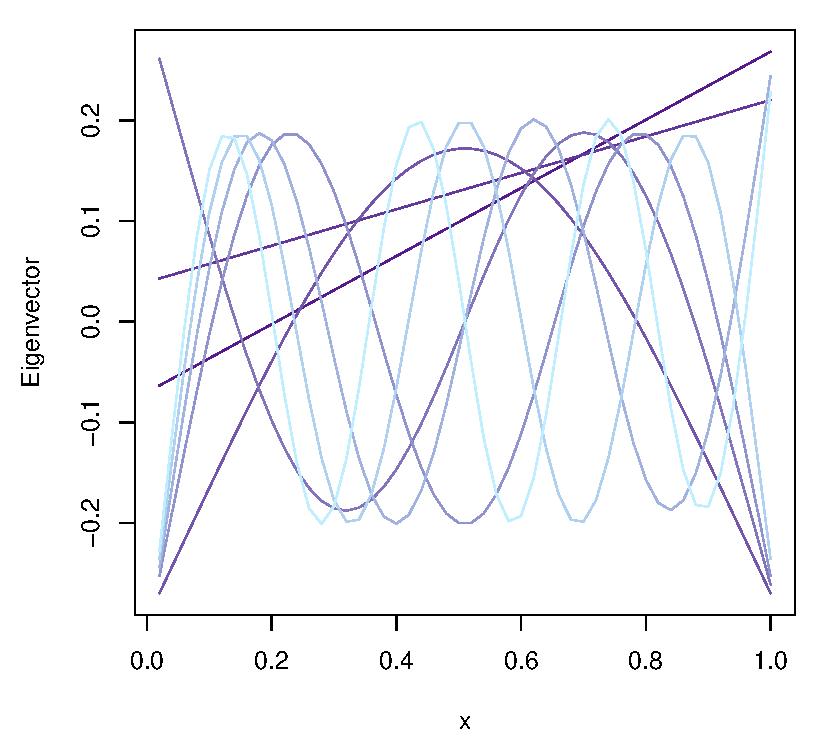
\includegraphics[width=0.495\textwidth]{reinsch_basis.pdf}
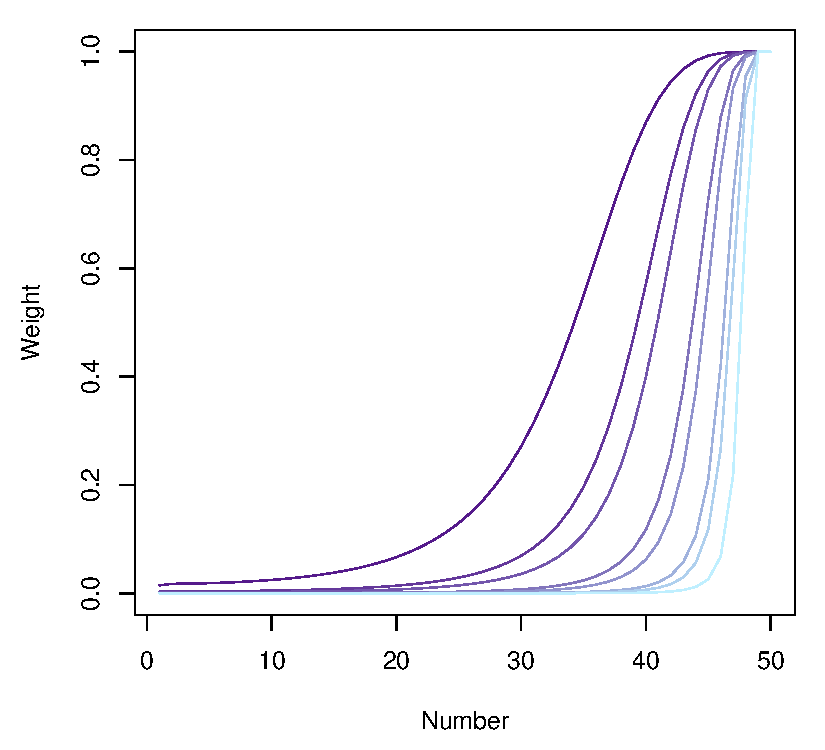
\includegraphics[width=0.495\textwidth]{reinsch_weight.pdf}
\caption{\it Insights from the Reinsch form of the cubic smoothing spline, for
  an example with $n=50$ input points. Left: the bottom 8 eigenvectors of $Q$,
  drawn using a color gradient where purple means the smallest eigenvalue, and
  light blue the largest eigenvalue. We see that smoother eigenvectors
  correspond to lower eigenvalues. Right: the shrinkage weights
  $w_j=1/(1+\lambda \sigma_j)$, $j=1,\dots,n$ for 8 values of $\lambda$, again
  drawn using a color gradient where purple means the largest $\lambda$, and
  light blue the smallest $\lambda$. For larger $\lambda$, the weights decay
  faster, so the smoothing spline estimator more strongly filters out wiggly
  components.}         
\label{fig:reinsch}
\end{figure}

\subsection{Equivalent kernel}

Recall that we can write a smoothing spline prediction as \smash{$\hf(x) = 
  w(x)^\T Y$}, for a weight function  $w(x) = (w_1(x), \dots, w_n(x)) \in \R^n$.
We know the analytic form of this weight function, but how about its qualitative
behavior? To be more precise, if we denote each component function by $w_i(x) =
w(x, x_i)$ to emphasize that this weight gets attributed to $(x_i, y_i)$ in the
weighted sum \smash{$w(x)^\T Y = \sum_{i=1}^n w(x, x_i) y_i$} which gives us the
smoothing spline prediction at $x$, then we can ask the following questions:         
\begin{itemize}
\item What shape does $z \mapsto w(x, z)$ have? Is it kernel-like?
\item Does this shape change as we vary the test point $x$? 
\end{itemize}

It's easy to just read off the answers to these questions from the rows of the
smoother matrix $S = N(N^\T N + \lambda \Omega)^{-1} N^\T$, since in our
expanded notation, its elements are
\[
S_{ij} = w_j(x_i) = w(x_i, x_j).
\]
Now, something very interesting happens when we plot a few rows of $S$. For
evenly-spaced inputs, they look like the translations of the same kernel: see
the left panel of Figure \ref{fig:ss_kernel}. Even more interestingly, for
unevenly-spaced inputs, the rows still have a kernel shape but now the bandwidth
appears to adapt to the density of the input points: lower density, larger
bandwidth. See the right panel of Figure \ref{fig:ss_kernel}.

\begin{figure}[tb]
\centering
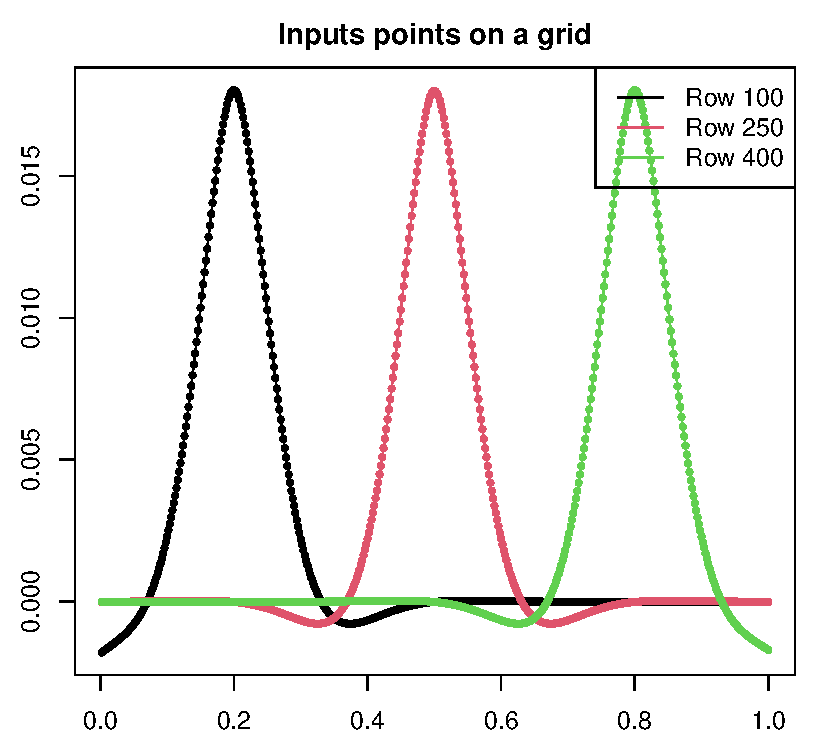
\includegraphics[width=0.495\textwidth]{ss_kernel1.pdf}
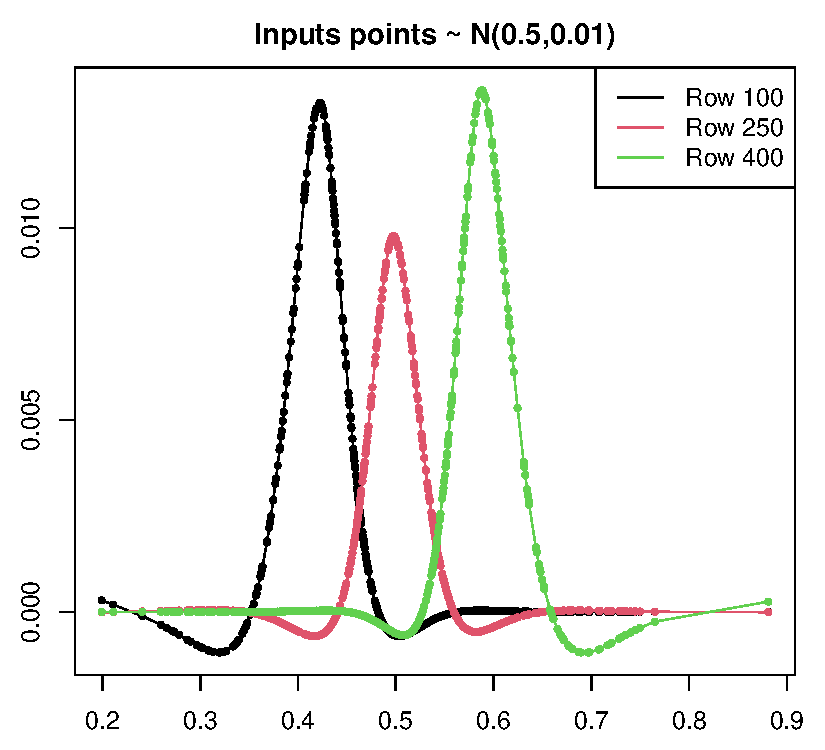
\includegraphics[width=0.495\textwidth]{ss_kernel2.pdf}
\caption{\it Three sample rows of the cubic smoothing spline operator $S$
  defined over $n=500$. Left: evenly-spaced inputs on a grid. The weights look
  like they are given by translations of the same kernel. Right: inputs drawn
  i.i.d.\ from $N(0.5, 0.01)$. The weights still look like kernels, but the
  bandwidth is now larger in low-density regions of the input domain.}     
\label{fig:ss_kernel}
\end{figure}

What we are seeing is an empirical validation of a beautiful asymptotic result
by \citet{silverman1984spline}, who proved that the cubic smoothing spline
estimator is asymptotically equivalent to a kernel regression estimator, with an 
unusual choice of kernel. Specifically, under suitable regularity conditions, we
have the large $n$ approximation,\footnote{Silverman actually shows that
  \smash{$w(x, z) \approx \frac{1}{h(z)} \frac{1}{p(z)} K( \frac{x-z}{h(z)})$},
  but the version we are stating has a more natural interpretation with respect
  to Figure \ref{fig:ss_kernel}, and is a consequence of symmetry of the
  smoother matrix $S$.}  
\[
w(x, z) \approx \frac{1}{h(x)} \frac{1}{p(x)} K\bigg( \frac{x-z}{h(x)} \bigg), 
\]
where $K$ is the ``Silverman kernel'': 
\[
K(t) = \frac{1}{2} \exp(-|t|/\sqrt{2}) \sin(|t|/\sqrt{2} + \pi/4), 
\]
and we have the local bandwidth: 
\[
h(x) = \bigg[ \frac{\lambda}{p(x)} \bigg]^{1/4},
\]
where $p(x)$ is the density of the input distribution at $x$. That is, the
bandwidth adapts to the local distribution of inputs. 

The Silverman kernel is ``kind of'' a higher-order kernel. It satisfies 
\[
\int K(t) \, dt = 1, \quad
\int t^j K(t) \, dt = 0, \; j=1,\dots,3, 
\quad \text{but} \quad 
\int t^4 K(t) \, dt = -24.
\]
So it lies outside the scope of usual kernel analysis. There is a lot more work
building off of Silverman's initial work that connects smoothing splines to
equivalent kernels. 

\section{Analysis tools}

Compared to that for kNN and kernel smoothing, the error analysis for smoothing
splines is a good deal more nuanced. Hence we'll dedicated an entire section to
learning the tools behind it. The upshot is that we'll be learning a basic
framework that can be used to analyze numerous other nonparametric estimators
(such as other penalized empirical risk minimizers).  

\subsection{Sobolev theory*}

We'll begin by introducing Sobolev spaces. This material can be mostly skipped
without interrupting the flow of understanding the main ideas in the rest of
this lecture, thus the asterisk. Well actually, you should probably read the
definition of weak differentiability, but you can treat the rest as
optional. Yes, optional, but also super interesting and fairly fundamental in
many ways, which is why we include some of the core details of Sobolev spaces 
here. To learn more, an excellent reference is \citet{evans2010partial}. 

\subsubsection{Weak derivatives}

First we introduce what is known as \emph{weak differentiability}. A function $f
: U \to \R$, where $U \subseteq \R^d$ is an open set, is called weakly
differentiable provided that there is some function $g : U \to \R^d$ such that
\begin{equation}
\label{eq:weak_derivative}
\int_U f(x) D \phi(x) \, dx = - \int_U g(x) \phi(x) \, dx,
\quad \text{for all $\phi \in C_c^\infty(U)$}, 
\end{equation}
where $C_c^\infty(U)$ is the set of all infinitely differentiable functions with
compact support in $U$, and $D\phi$ is the derivative of one such function
$\phi$. The function $g$ satisfying \eqref{eq:weak_derivative} is unique almost
everywhere, and denoted by $Df$ henceforth, called the weak derivative of $f$.

The motivation for this definition of weak differentiability is integration by
parts: if $f,\phi$ are differentiable in the classical (usual) sense, then
\smash{$\int_U f(x) D \phi(x) \, dx = - \int_U Df(x) \phi(x) \, dx$} by
integration by parts (applied componentwise), where there are no boundary terms
because $\phi$ has compact support. Thus, we define the weak derivative $g = Df$
such that this holds for all infinitely differentiable compactly-supported
$\phi$.

Higher-order derivatives follow similarly. For a multi-index
$\alpha=(\alpha_1,\dots,\alpha_d) \in \Z^d_+$, recall, we write $|\alpha| =
\alpha_1 + \cdots + \alpha_d$ and we denote  
\[
D^\alpha \phi = \frac{\partial^{|\alpha|} \phi}{\partial x_1^{\alpha_1} \partial 
  x_2^{\alpha_2} \dots \partial x_d^{\alpha_d}},
\]
interpreted in the classical (usual) sense for a function $\phi$. In the weak
sense, $f$ is said to have $\alpha\th$ weak differentiable $g$ if 
\begin{equation}
\label{eq:weak_derivative_alpha}
\int_U f(x) D^\alpha \phi(x) \, dx = - (1)^{|\alpha|} \int_U g(x) \phi(x) \, dx,
\quad \text{for all $\phi \in C_c^\infty(U)$}.   
\end{equation}
Again, the function $g$ satisfying \eqref{eq:weak_derivative_alpha} is unique
almost everywhere, and we denote by $D^\alpha f$.

Of course, the weak derivative reduces to the classical derivative exists when
the latter exists. However, weak differentiability is more general. An example
of a function that is weakly differentiable but not classically differentiable
is
\[
f(x) = x_+, \quad \text{with weak derivative $Df(x) = 1\{x > 0\}$.} 
\]
An example of a function that is \emph{not} weakly differentiable is $f(x) =
1\{x > 0\}$. For this, one can check that the condition
\eqref{eq:weak_derivative} cannot hold: taking $\phi$ to be any function whose
support includes 0, we learn that
\[
\phi(0) = \int g(x) \phi(x) \, dx.
\]
This cannot possibly be true for all infinitely differentiable $\phi$. This
cannot possibly be true for all $\phi$ unless $g=0$. But if $g=0$, then we
cannot recover $\phi(0)$ through integration, since the right-hand side above
will always be 0.   

\subsubsection{Sobolev spaces}

We are now equipped to define what are called \emph{Sobolev spaces}. In what
follows it'll be simplest to take the domain $U$ to be bounded, so let's 
assume that henceforth (though to be clear it is by no means necessary). For an
integer $k \geq 0$, and $1 \leq p \leq \infty$, we define the Sobolev space    
\[
W^{k,p}(U) = \Big\{ f : U \to \R \,:\, \text{$D^\alpha f$ exists in the weak
  sense, and $\|D^\alpha f\|_p < \infty$ for all $|\alpha| \leq k$} \Big\}. 
\]
Here $\|\cdot\|_p$ denotes the $L^p$ norm on $U$: \smash{$\|f\|_p = (\int_U
  |f(x)|^p \, dx)^{1/p}$ for $p < \infty$} and \smash{$\|f\|_\infty = \esssup_{x 
  \in U} \, |f(x)|$}.

Sobolev spaces are central in the study of partial differential equations, which
is commonly where you'll find people (mathematicians) referring to them. But
they also play an important role in nonparametric statistics. For example, if
you recall the smoothing spline problem \eqref{eq:ss}, where we said that ``the  
minimization is all functions $f$ for the which the criterion is well-defined
and finite'', the domain here can actually be viewed as the Sobolev
space\footnote{We'll ignore here, and in several other places, the fact that the 
  domain is closed. Recall, we defined Sobolev spaces on open domains, and we  
  will do the same for H{\"o}lder spaces as well. Hence, we are being slightly 
  imprecise by abruptly allowing closed domains but it's easiest to do so for
  simplicity of exposition.}  
\[
W^{m,2}([a,b]) = \Big\{ f : [a,b] \to \R \,:\, \text{$D^m f$ exists in the weak
  sense, and $\|D^m f\|_2^2 = \int_a^b [D^m f(x)]^2 \, dx < \infty$} \Big\}. 
\]

We note that, generally speaking, when working in Sobolev spaces (just like
$L^p$ spaces), we identify two functions that are equal almost everywhere. In 
other words, each element $f$ in a Sobolev space is really an equivalence class
of functions, any pair of which agree except on a set of measure zero.

Now we recall \emph{H{\"o}lder spaces}. We touched on these in the lecture on 
kernels. Formally, for an integer $r \geq 0$, and $0 < \gamma \leq 1$, we define
the H{\"o}lder space
\begin{multline*}
C^{r+\gamma}(U) = \Bigg\{ f : U \to \R \,:\, \text{$D^\alpha f$ exists,
  $\|D^\alpha f\|_\infty < \infty$ for all $|\alpha| \leq r$, and} \\   
  \sup_{x \not= z} \, \frac{|D^\alpha f(x) - D^\alpha f(z)|}{\|x-z\|_2^\gamma} < 
  \infty \; \text{for all $|\alpha| = r$} \bigg\}.   
\end{multline*}
In the above, we can interpret $D^\alpha f$ to mean a classical derivative, but
as we'll discuss just below, we can also identify the H{\"o}lder space with a
particular Sobolev space. 

Let's pause to examine the relationship between the Sobolev space
$W^{k,\infty}(U)$ and the H{\"o}lder space $C^k(U)$. The former contains all
functions $f$ such that the $\alpha\th$ weak derivative of $f$ is bounded for
all $|\alpha| \leq k$. The latter contains all functions $f$ such that the
$\alpha\th$ derivative of $f$ is bounded for all $|\alpha| < k$, and $D^\alpha
f$ Lipschitz for $|\alpha| = k$. It turns out that these two conditions are
really saying the same thing, and we can identify $W^{k,\infty}(U)$ with
$C^k(U)$. To be precise,  in doing so, we identify each $f$ in the Sobolev space
with its classically differentiable version.

Much more can be said about the connection between Sobolev and H{\"o}lder
spaces, which is covered next.

% Theorem 4 in Chapter 5.8 of Evans (2010), requires \partial U to be C^1

\subsubsection{Embedding theorems}

Among the whole optional part of material on Sobolev spaces, this next bit   
really is the \emph{most} optional, but it's too cool not to cover. We start by
defining norms on Sobolev and H{\"o}lder spaces; namely,
\[
\|f\|_{W^{k,p}(U)} = 
\begin{dcases} 
\Bigg( \sum_{|\alpha| \leq k} \|D^\alpha f\|_p^p \Bigg)^{1/p} & \text{if $p <
  \infty$} \\
\;\;\; \sum_{|\alpha| \leq k} \|D^\alpha f\|_\infty & \text{if $p = \infty$}   
\end{dcases}
\qquad \text{for $f \in W^{k,p}(U)$},
\]
and 
\[
\|f\|_{C^{r+\gamma}(U)} = \sum_{|\alpha| \leq r} \|D^\alpha f\|_\infty +
\sum_{|\alpha| = r} \sup_{x \not= z} \, \frac{|D^\alpha f(x) - D^\alpha f(z)|} 
{\|x-z\|_2^\gamma}
\qquad \text{for $f \in C^{r+\gamma}(U)$}. 
\] 
Equipped with these norms, $W^{k,p}(U)$ and $C^{r+\gamma}(U)$ are Banach 
spaces (complete normed linear spaces). In fact, when $p=2$, the space
$W^{k,p}(U)$ is a Hilbert space (complete inner product space) under the inner
product \smash{$\langle f, g \rangle_{W^{k,p}(U)} 
= \sum_{|\alpha| \leq k} \langle D^\alpha f, D^\alpha g \rangle_2 
= \sum_{|\alpha| \leq k} \int_U D^\alpha f(x) D^\alpha g(x) \, dx$.}

Now here comes the cool part, which are special inequalities\footnote{In an
  unfortunate clash of nomenclature with statistics, you'll often hear
  mathematicians calling these ``estimates''.} involving Sobolev norms that lead 
to what are known as \emph{embedding theorems}. There are really several
embedding theorems that were developed over many years, by different authors
(Gagliardo, Nirenberg, Sobolev, Morrey, others), but now the totality of them is
usually just called ``the Sobolev embedding theorem''. In a nutshell, this is
what it says (recall that $d$ refers to the dimension of the domain $U$, which
is assumed to be an open bounded subset of $\R^d$). 

\paragraph{The case $pk < d$, subcritical regime.}

In this case we a have lower smoothness-to-dimension ratio. Let $0 \leq \ell <
k$ be an integer, and $p < q < \infty$, such that the pair satisfies   
\[
\frac{1}{q} - \frac{\ell}{d} = \frac{1}{p} - \frac{k}{d}.
\]
Then we have, for a constant $C>0$ depending only on $k,p,\ell,q$ and $U$, 
\[
\|f\|_{W^{\ell,q}(U)} \leq C \|f\|_{W^{k,p}(U)}, \quad \text{for all $f \in
  W^{k,p}(U)$}.
\]
This means that $W^{k,p}(U) \subseteq W^{\ell,q}(U)$, and moreover we have what 
is known as a \emph{continuous embedding} of normed spaces. From the above    
inequality, we learn that any norm ball of radius $\rho$ in the former space
is contained in a normal ball of the latter, whose radius is at most $C\rho$.

Note that in the special case where we take $\ell = 0$, we get that for  
\[
q = \frac{pd}{d-pk},
\]
and a constant $C>0$ depending only on $k,p,q$ and $U$, it holds that 
\[
\|f\|_q \leq C \|f\|_{W^{k,p}(U)}, \quad \text{for all $f \in W^{k,p}(U)$}. 
\]
This means that $W^{k,p}(U) \subseteq L^q(U)$, and the embedding is continuous.  

% Theorems 2 and 6 in Chapter 5.6 of Evans (2010), requires \partial U to be 
% C^1, doesn't actually state the result for general \ell, only for \ell = 0  

\paragraph{The case $pk > d$, supercritical regime.}

In this case we a have higher smoothness-to-dimension ratio. Let $0 \leq r < k$
be an integer, and $0 < \tau \leq 1$, such that the pair satisfies 
\[
\frac{r+\tau}{d} = \frac{k}{d} - \frac{1}{p}.
\]
A technical detail: if the value of $r,\tau$ satisfying the above results in
$\tau = 1$, then we need to ``downgrade'' it to a value less than 1. That is,
let $\gamma = \tau$ if $\tau < 1$, and otherwise let $0 < \gamma < 1$. Then we
have, for a constant $C>0$ depending only on $k,p,r,\gamma$ and $U$,       
\[
\|f\|_{C^{r+\gamma}(U)} \leq C \|f\|_{W^{k,p}(U)}, \quad \text{for all $f \in
  W^{k,p}(U)$}. 
\]
This means that $W^{k,p}(U) \subseteq C^{r+\gamma}(U)$, and the embedding is
continuous. In view of this, we can always identify each function $f \in
W^{k,p}(U)$ with its $r$ times classically differentiable version.     

% Theorems 5 and 6 in Chapter 5.6 of Evans (2010), requires \partial U to be
% C^1, doesn't quite state the result the same way as we do

\medskip
(The critical regime $pk = d$ is actually a bit more subtle and we'll skip over
it.)  

How do we interpret the Sobolev embedding theorem? In the subcritical regime, it
says that we can trade off smoothness in the differential sense with smoothness
in the integral sense. Given a $k$ times (weakly) differentiable function, whose
derivatives are in $L^p(U)$, the embedding theorem tells us that its derivatives
of order $\ell < k$ are less ``peaky'' and more ``evenly spread out'', since
they are $L^q(U)$ with $q > p$.

In the supercritical regime, the conclusion is arguably even more
fascinating---it says that knowing a function's derivatives are smooth in a
global (integrated) sense tells us something about local smoothness of lower
order derivatives, at each point in the domain. Given a $k$ times (weakly)
differentiable function, the embedding theorem starts off with a statement about
the size of \smash{$\sum_{|\alpha| \leq k} \int_U |D^\alpha f(x)|^p \, dx$}, and
translates this into a statement about the H{\"o}lder constant of $D^\alpha f$
for $|\alpha| < k$.      

Figure \ref{fig:sobolev} gives an illustration of the tradeoffs navigated by the
Sobolev embedding theorem (the plots that are shown are sometimes called
``DeVore diagrams'' in honor of Ron DeVore).  

\begin{figure}[tb]
\centering
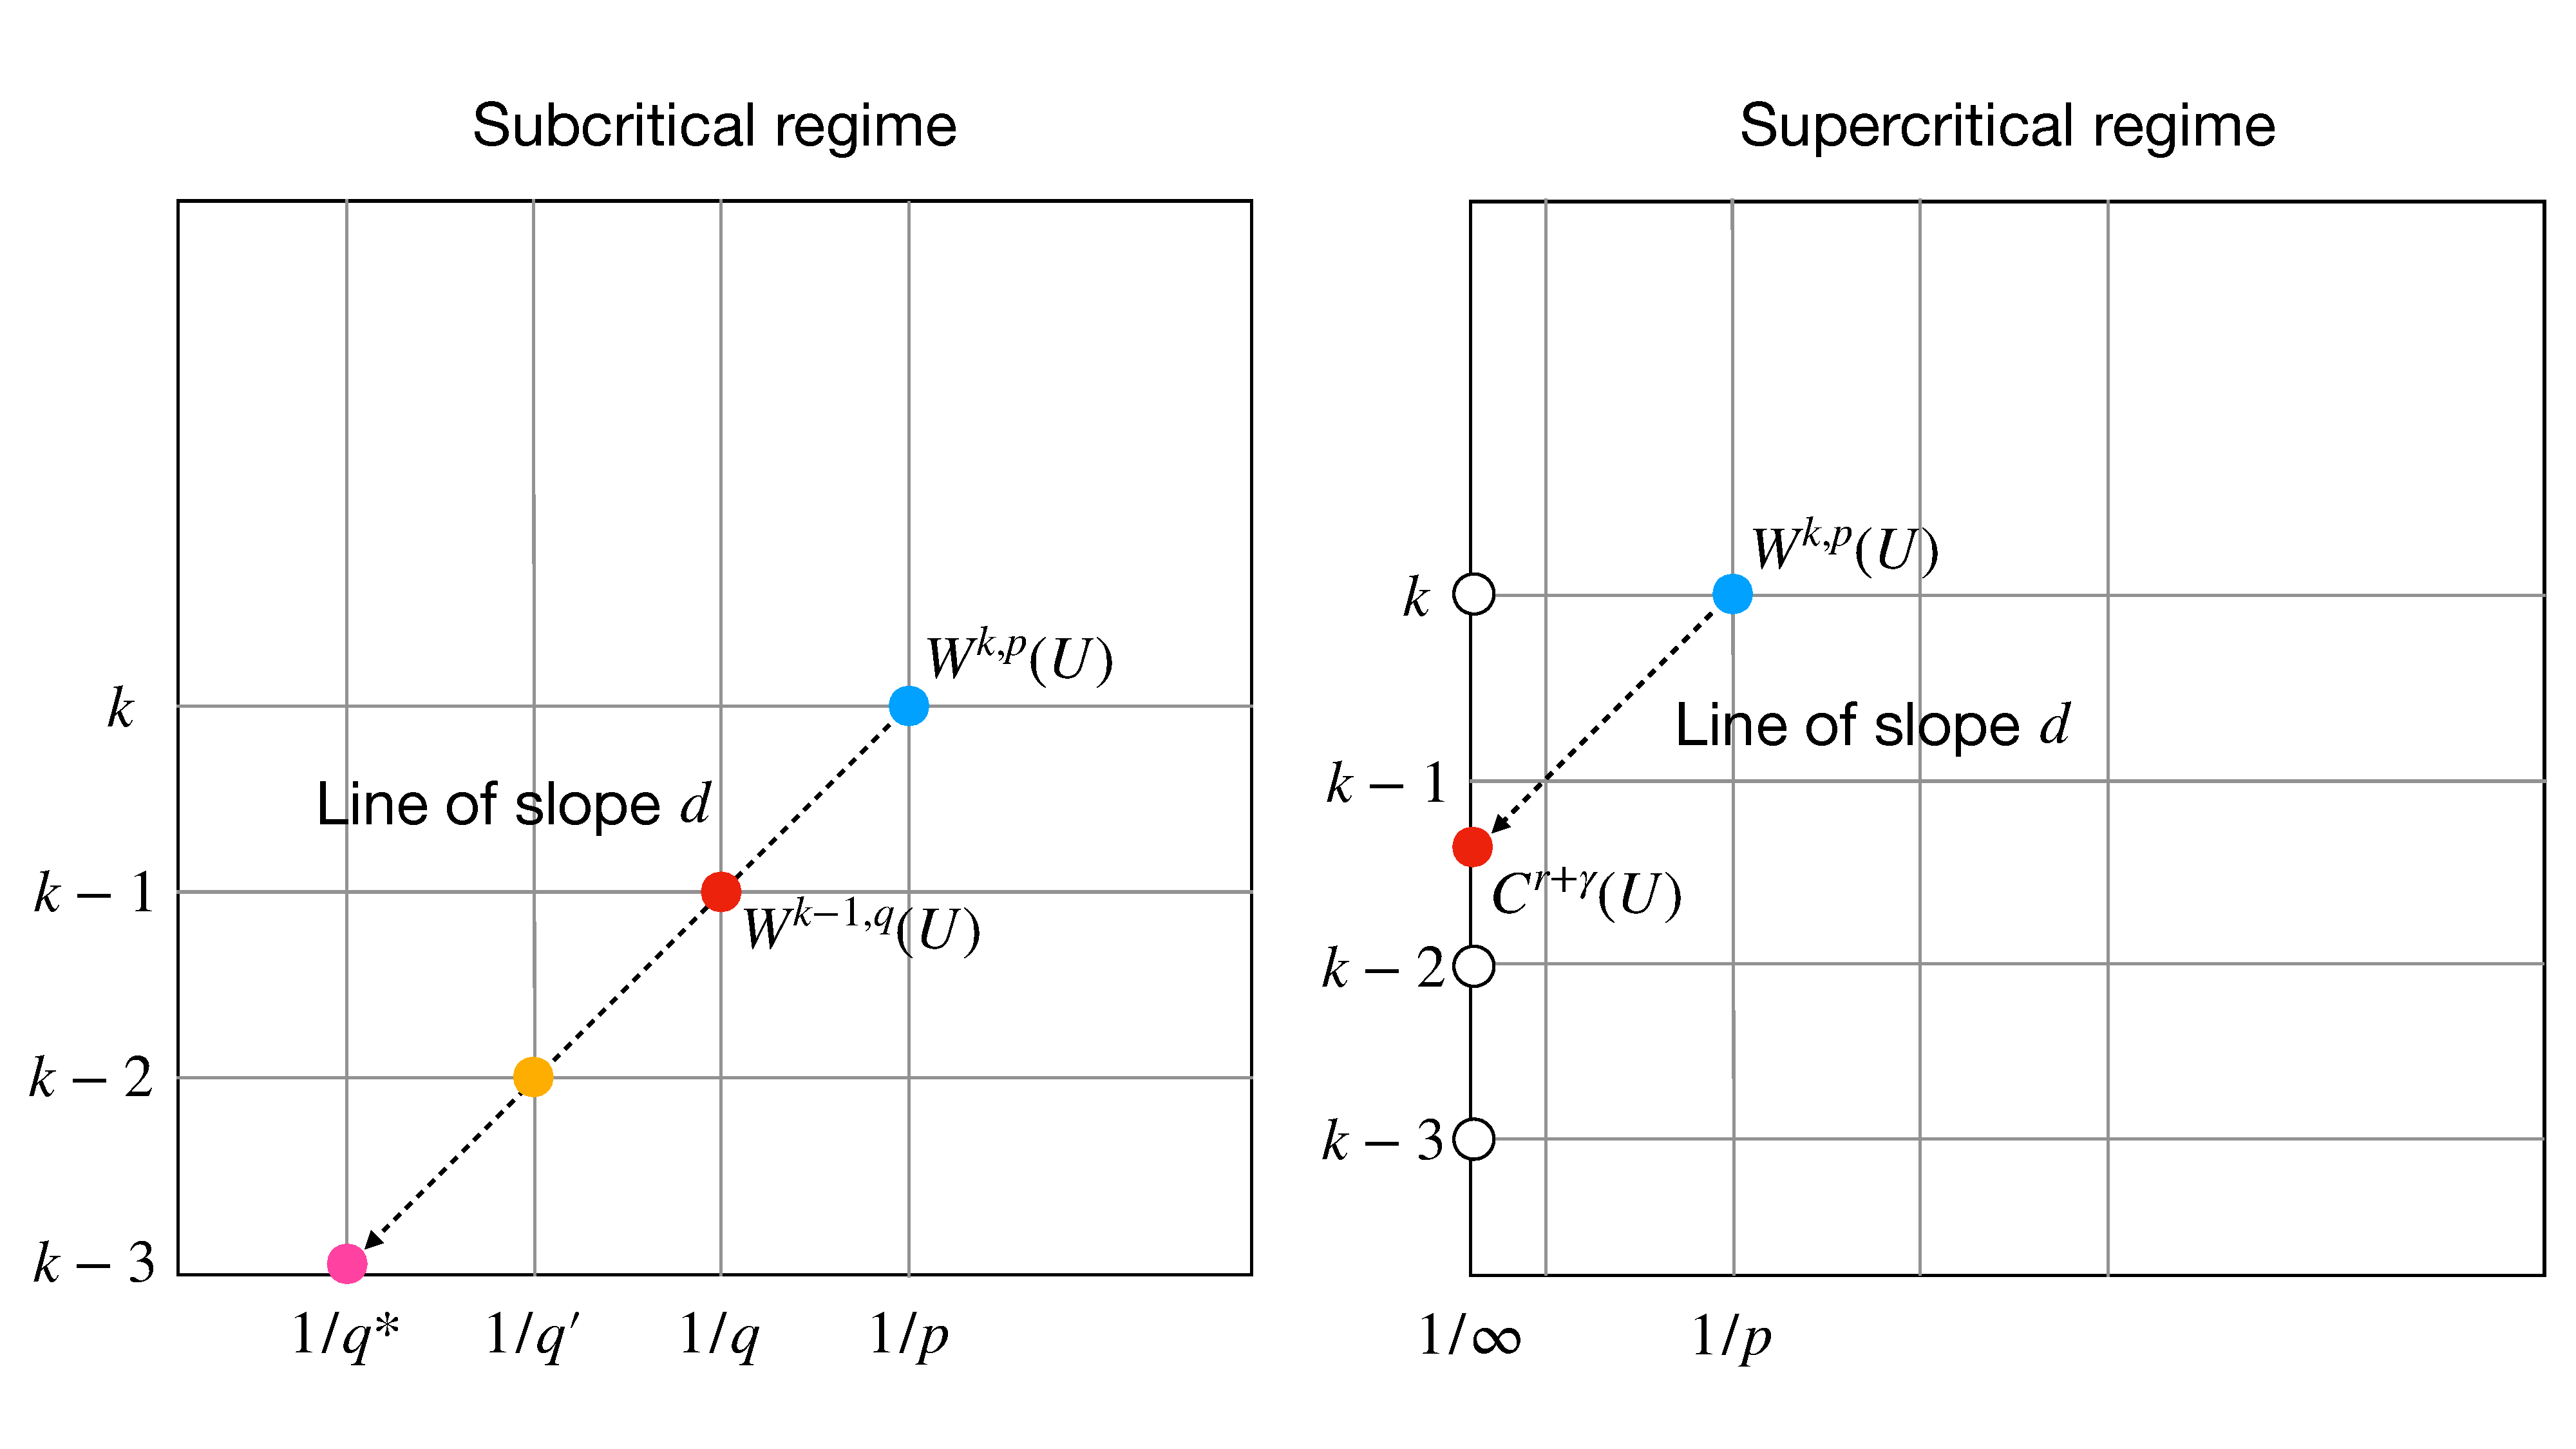
\includegraphics[width=\textwidth]{sobolev.pdf}
\caption{\it Illustrations of the Sobolev embedding theorem. In each plot, we 
  parametrize the x-axis by $1/p$ and the y-axis by $k$. Hence, as we move
  right-to-left, we increase the index of the $L^p$ norm that is used to measure 
  integral smoothness, and functions get less ``locally peaked'' and more 
  ``evenly spread out''. As we move top-to-bottom, we decrease the number of
  (weak) derivatives under consideration. Left: subcritical regime with $pk <
  d$. We traverse a line of slope $d$, moving down and to the left, in order to
  visit the different Sobolev spaces into which $W^{k,p}(U)$ embeds, culminating
  in an intersection with the x-axis ($k=0$) at $q = pd/(d-pk)$. Right:
  supercritical regime with $pk > d$. Similarly, we traverse a line of slope $d$
  to find the H{\"o}lder space into which $W^{k,p}(U)$ embeds, which is given by
  an intersection with the y-axis ($q = \infty$). The open white circles denote
  cases in which the embedding fails for $\gamma = 1$.}  
\label{fig:sobolev}
\end{figure}

\subsection{Empirical process theory}

\def\Rad{\mathrm{Rad}}

Next we cover some important concepts and probabilistic tools from empirical
process theory. We cover this material in a more utilitarian manner than our
treatment of Sobolev theory. That is, we will mostly just stick to the details
needed to understand the error analysis to come in the next section. A lot more
can be said; two excellent references on the subject are
\citet{vandegeer2000empirical, wainwright2019high}.    

\subsubsection{Entropy and Rademacher complexity} 

\def\diam{\mathrm{diam}}

Given a class of functions $\cF$, we define its \emph{metric entropy} (or simply   
entropy) as the logarithm of smallest number of balls in a norm $\|\cdot\|$ of
radius $\delta>0$ needed to cover $\cF$. This is denoted     
\[
\log N(\delta, \cF, \|\cdot\|), 
\]
and also referred to as its log covering number. A visualization is given in
Figure \ref{fig:covering}.

\begin{figure}[tb]
\centering
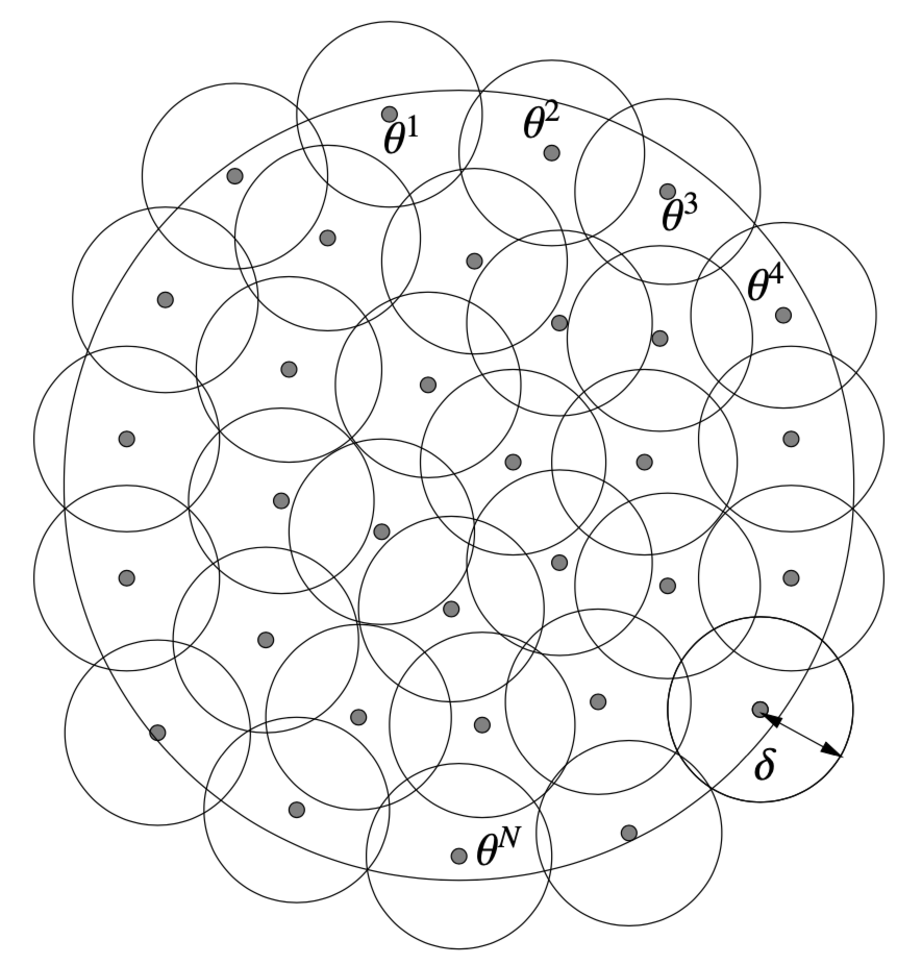
\includegraphics[width=0.45\textwidth]{covering.pdf}
\caption{\it Illustration of a covering using balls of radius $\delta$. The
  entropy is the logarithm of the smallest possible number of balls in such a
  covering. Credit: Chapter 5 of \citet{wainwright2019high}.}
\label{fig:covering}
\end{figure}

Seemingly unrelated, but actually connected idea, is Rademacher complexity. This
itself comes in two flavors. The \emph{empirical Rademacher complexity} based
on a sample $x_1,\dots,x_n$ is the expected largest absolute inner product
achievable with i.i.d.\ Rademacher noise $\sigma_1,\dots,\sigma_n$ (each of
which take on the value $\pm 1$ with equal probability). To be precise, this is 
defined as   
\[
\Rad(\cF, x_{1:n}) = \E \Bigg[ \sup_{f \in \cF} \, \frac{1}{n} \Bigg|
\sum_{i=1}^n \epsilon_i f(x_i) \Bigg| \Bigg]. 
\]
The expectation above is over $\sigma_1,\dots,\sigma_n$ with $x_1,\dots,x_n$
fixed. Meanwhile, we can then just define \emph{population Rademacher
  complexity} as the expected value of the empirical Rademacher complexity,   
\[
\Rad(\cF) = \E\big[ \Rad(\cF, x_{1:n}) \big],
\]
over i.i.d.\ draws $x_1,\dots,x_n$ from some input distribution.

A general result connecting these two notions of complexity is called
\emph{Dudley's entropy integral}, which we can state as follows. Denote by
$B_n(\rho)$ the ball in the norm $\|\cdot\|_n$ (the empirical norm based on the
sample $x_1,\dots,x_n$) of radius $\rho$ centered at the origin. Then there
exists a constant $C>0$ such that
\begin{equation}
\label{eq:dudley}
\Rad(\cF \cap B_n(\rho), x_{1:n}) \leq \frac{C}{\sqrt{n}} \int_0^\rho
\sqrt{\log N(\delta, \cF, \|\cdot\|_n)} \, d \delta.
\end{equation}

% Example 5.24 in Chapter 5.3 of Wainwright (2019)

Entropy and Rademacher complexity are each interesting and important, and have
several applications in probability and nonparametric analysis, but for our
purposes, we can think of them as follows. Entropy arises naturally in a
probabilistic technique known as chaining. This can be used to control
sub-Gaussian processes; in particular, it can be used to bound what is known as
the sub-Gaussian complexity   
\[
\sup_{f \in \cF} \, \Bigg| \frac{1}{n} \sum_{i=1}^n \epsilon_i f(x_i) \Bigg|, 
\]
where $\epsilon_1,\dots,\epsilon_n$ are i.i.d.\ mean zero sub-Gaussian random
variables. We'll see this quantity arising naturally in our error analysis of
smoothing splines, and we'll see the role entropy plays in Lemma
\ref{lem:sg_complexity} below. 

On the other hand, Rademacher complexity appears when using a technique called
symmetrization, and other techniques, to analyze the fluctuations of empirical
averages around their population means. For us, we will see it can be used to
control the difference between the empirical $\|\cdot\|_n$ and population
$\|\cdot\|_2$ norms, with high probability (over the draws of
$x_1,\dots,x_n$). We'll see this in Lemma \ref{lem:norm_coupling} below.     

Lastly, we remark that we are commonly interested in (an upper bound on) how
$\log N(\delta, \cF, \|\cdot\|_n)$ scales with $\delta$, as $\delta \to 0$, and
since we are considering here the empirical norm $\|\cdot\|_n$, we ideally want
log covering number bounds that hold for any arrangement of
$x_1,\dots,x_n$. This can be upper bounded by considering $\log N(\delta, \cF,
\|\cdot\|_\infty)$ (because $\|f-g\|_\infty \leq \delta$ implies $\|f-g\|_n \leq
\delta$). Table \ref{tab:entropy} gives entropy rates for a few example function
classes of interest. 

\begin{table}[tb]
\centering
\renewcommand{\arraystretch}{1.5}
\begin{tabular}{p{3in}|c|c}
Function class $\cF$ & Norm $\|\cdot\|$ & Entropy rate \\ \hline \hline 
$r$-dimensional (e.g., class of natural splines with $r$ knots) with $\diam(\cF,
  \|\cdot\|_n) = \rho$ & $\|\cdot\|_n$ & $r \log(\rho/\delta)$ \\ \hline
% Example 5.8 in Chapter 5.1 of Wainwright (2019)
$L$-Lipschitz functions on $[0,1]^d$ & $\|\cdot\|_\infty$ & $(L/\delta)^d$
  \\ \hline
% Example 5.10 in Chapter 5.1 of Wainwright (2019)
$m$-times weakly differentiable functions on $[0,1]$ such that $\int_0^1 
[D^m f(x)]^2 \, dx \leq L$ and $\|f\|_\infty \leq M$, where $m \geq 2$ & 
$\|\cdot\|_\infty$ & $(L/\delta)^{1/m} + \log(M/\delta)$ \\ \hline 
% Birman and Solomyak (1967)
Weakly differentiable functions on $[0,1]$ such that $\int_0^1 [f'(x)]^2 \, dx 
  \leq L$ and $\|f\|_\infty \leq M$ & $\|\cdot\|_2$ & $L/\delta + 
  \log(M/\delta)$  
% Birman and Solomyak (1967)
\end{tabular}
\caption{\it Entropy rates for some function classes of interest in
  nonparametric analysis.} 
\renewcommand{\arraystretch}{1}
\label{tab:entropy}
\end{table}

\subsubsection{Sub-Gaussian random variables}

\emph{Sub-Gaussianity} is a condition that captures some of the key properties
of the Gaussian tail (but at the same time accomodates many distributions that
are not Gaussian).   

A random variable $X$ is said to be sub-Gaussian with mean $\mu$ and
variance proxy $\sigma^2>0$ if   
\[
\E[ e^{t (X - \mu)} ] \leq e^{\sigma^2 t^2 / 2}, \quad \text{for all $t \in
  \R$}. 
\]
This says that the moment generating function of $X$ is dominated by the moment
generating function of $N(\mu, \sigma^2)$ random variable.

Here are some examples of sub-Gaussian random variables.

\begin{itemize}
\item A $N(\mu, \sigma^2)$ random variable. 
\item A bounded random variable. Hence e.g., Rademacher, Bernoulli, and binomial   
  random variables are all sub-Gaussian.
\item A random variable $X$ for which all even moments exist and satisfy  
\[
\E[X^{2k}] \leq \frac{(2k)!}{2^k k!} \theta^{2k}, \quad \text{for all
  $k=1,2,3,\dots$},
\]
for some parameter $\theta \geq 0$. In fact this moment condition is equivalent
to sub-Gaussianity.   
% Theorem 2.6 (III) in Section 2.1 of Wainwright (2019)
\end{itemize}

An example of a random variable that is not sub-Gaussian is a Poisson random
variable with any mean $\mu$ (this is instead \emph{sub-exponential}, which is a 
weaker condition).

\paragraph{Tail bound for averages.}

An important fact about sub-Gaussian random variables is that they admit a 
Bernstein-type tail bound: if $X_i$, $i=1,\dots,n$ are independent sub-Gaussian
random variables, with each $X_i$ having mean zero and variance proxy
$\sigma_i^2$, then for all $t>0$,    
\[
\P(\bar{X}_n \geq t) \leq \exp \bigg( \frac{-nt^2}{
    \frac{1}{n}\sum_{i=1}^n \sigma_i^2} \bigg),
\]
where \smash{$\bar{X}_n = \frac{1}{n} \sum_{i=1}^n X_i$}. We can also get a
two-sided bound where we multiply right-hand side above by 2 (since $X$ is mean
zero sub-Gaussian with variance proxy $\sigma^2$ if and only if $-X$ is).    

\paragraph{Tail bound for maxima.}

Another useful fact about sub-Gaussian random variables is that maximum of a
large number of them sharply concentrates: if $X_i$, $i=1,\dots,n$ are sub-Gaussian
random variables, which need not be independent, and each $X_i$ has mean zero
and variance proxy $\sigma^2$, then for all $t>0$,    
\[
\P \bigg(\max_{i=1,\dots,n} \, X_i \geq \sigma \sqrt{2 (\log n + t)} \bigg) 
\leq e^{-t}.  
\]
It also holds that
\[
\E \bigg[ \max_{i=1,\dots,n} \, X_i \bigg] \leq \sigma \sqrt{2 \log n}.
\]

\paragraph{Tail bound for quadratic forms.}

A last useful fact we will cite about sub-Gaussian random variables concerns
tail concentration for quadratic forms: if $X_i$, $i=1,\dots,n$ are independent
sub-Gaussian random variables, with each having mean zero and variance proxy 
$\sigma^2$, then for any positive semidefinite matrix $Q \in \R^{n \times n}$
and all $t>0$,    
\begin{equation}
\label{eq:sg_quadratic}
\P\Big( X^\T Q X \geq \sigma^2 \big[ \tr(Q) + 2 \|Q\|_F \sqrt{t} + 2
\|Q\|_{\mathrm{op}} \, t \big] \Big) \leq e^{-t},
\end{equation}
where $X = (X_1,\dots,X_n) \in \R^n$ is the vector of sub-Gaussian variates, so 
that \smash{$ X^\T Q X = \sum_{i,j=1}^n Q_{ij} X_i X_j$}, and \smash{$\|Q\|_F, 
\|Q\|_{\mathrm{op}}$} denote the Frobenius and operator norms of $Q$, 
respectively. The result we are stating here is from \citet{hsu2012tail}, which
is similar to the Hanson-Wright inequality (but has simple explicit constants).       

\subsubsection{Sub-Gaussian complexity bound}

We now turn to the most sophisticated and powerful empirical process theory 
result we've seen thus far.

\begin{lemma}[Adapted from Lemma 3.5 of \citealt{vandegeer1990estimating}] 
\label{lem:sg_complexity}
Let $\epsilon_i$, $i=1,\ldots,n$ denote independent sub-Gaussian random
variables, each having mean zero variance proxy $\sigma^2$. Let $J$ be a
seminorm on acting on functions from $U$ to $\R$, and denote its unit seminorm
ball by 
\[
B_J(1) = \{ f : U \to \R \,:\, J(f) \leq 1 \},
\]
Also denote \smash{$B_\infty(M) = \{ f : U \to \R \,:\, \|f\|_\infty \leq M
  \}$}, where $M>0$ is an arbitrary constant. Assume that for sufficiently small
$\delta>0$, there exists constants $0<w<2$ and $C>0$ such that     
\[
\sup_{x_1,\dots,x_n} \,
\log N\big(\delta, B_J(1) \cap B_\infty(1), \|\cdot\|_n \big) \leq C
\delta^{-w}. 
\]
Then there are constants $c_1,c_2,n_0>0$, depending only on
$\sigma,M,C,w$, such that for all $\gamma \geq c_1$ and $n \geq n_0$,        
\[
\sup_{x_1,\dots,x_n} \,
\sup_{f \in B_J(1) \cap B_\infty(M)} \,
\frac{\frac{1}{n} \sum_{i=1}^n \epsilon_i f(x_i)} 
{\|f\|_n^{1-w/2}} \leq \frac{\gamma}{\sqrt{n}}, 
\]
with probability at least $1-\exp(-c_2 \gamma^2)$.
\end{lemma}

To get a sense of what the result in the lemma gives us, let's rewrite the
conclusion a little differently: it says that uniformly over all $f$ with $J(f)
\leq 1$ and $\|f\|_\infty \leq M$, we have 
\[
\frac{1}{n} \sum_{i=1}^n \epsilon_i f(x_i) \leq \gamma \|f\|_n
\frac{\|f\|_n^{-w/2}}{\sqrt n},
\]
with high probability. Now think about what a simple application of
Cauchy-Schwartz would give us: 
\[
\frac{1}{n} \sum_{i=1}^n \epsilon_i f(x_i) \leq \|\epsilon\|_n \|f\|_n 
\leq c \|f\|_n,
\]
where the second inequality holds with high probability, for some constant  
$c>0$. Here we are abusing notation somewhat and denoting 
\smash{$\|\epsilon\|_n^2 = \frac{1}{n} \sum_{i=1}^n \epsilon_i^2$}; and for the
high probability statement we are (vaguely) referring to the concentration
result \eqref{eq:sg_quadratic} for a quadratic form of sub-Gaussians (with
\smash{$Q = \frac{1}{n} I$}). If we ignore the leading factors of $\gamma, c$,
then we see that the second-to-last display is better than the last display when  
\[
\frac{\|f\|_n^{-w/2}}{\sqrt n} \leq 1 \iff \|f\|_n \geq n^{-1/w}.
\]
That is, except for functions $f$ of really small empirical norm, we improve on
Cauchy-Schwartz, and dramatically so when $f$ is of larger empirical norm. For
example, when \smash{$\|f\|_n = n^{-1/(2+w)}$} (this is not an arbitrarily
chosen rate ... you'll see why we're interested in this a bit later, when we do
the error analyis), then the ``speedup'' we get from
Lemma \ref{lem:sg_complexity} is:
\[
\frac{\|f\|_n^{-w/2}}{\sqrt n} = n^{-1/(2+w)}.
\]

\subsubsection{Empirical and population norm coupling}

Coupling of empirical and population norms as in Lemma 15. 
We will need Theorem 14.1 of Wainwright. 

\begin{lemma}
\label{lem:norm_coupling}
\end{lemma}

Mention one-sided bound? As in Lemma 17

\section{Main analysis} 

\subsection{Basic inequality}

Derive the basic inequality. Remark that a more refined analysis at the start
can do better in terms of the constants, leading to what is known as an oracle 
inequality, and we'll see this later when we analyze the lasso.  

\subsection{Localization}

Interlude on how complexity combined with an population or empirical norm bound
gives you a sup norm bound. Statement similar to Lemma 7
\[
\|f\|_\infty \leq R_1 \|f\|_n + R_2 J(f)
\]
and also similar to Lemma 16
\[
\|f\|_\infty \leq R_1 \|f\|_2 + R_2 J(f)
\]
Yes! This is right, I think just look at the proof of Lemma 7

\subsection{Sub-Gaussian control}

\subsection{Approximation error}

\subsection{An example theorem}

% Notes to me ... think about how we want to define $W^{k,p}(L; U)$. Just in
% terms of the Sobolev seminorm? I think so. But then acknowledge that this is a 
% bit different from how we do things in Sobolev theory. Same with Holder
% spaces. Make this a long footnoote. 

\section{Multivariate splines}

\section{RKHS methods}

\section{Linear smoothers}

\bibliographystyle{plainnat}
\bibliography{../../common/ryantibs.bib}

\clearpage
\appendix

\section{B-splines}
\label{app:bs}

Note: this appendix is pretty much taken shamelessly from Appendix C of 
\citet{tibshirani2022divided}.

Though the truncated power basis \eqref{eq:tpb} is the simplest basis for
splines, the B-spline basis is just as fundamental, and it was ``there at the 
very beginning'', appearing in Schoenberg's original paper on splines
\citep{schoenberg1946contributions1}. Here we are quoting
\citet{deboor1976splines}, who gives a masterful survey of the history and
properties of B-splines (and points out that the name ``B-spline'' is derived
from Schoenberg's use of the term ``basic spline'', to further advocate for the
idea that B-splines can be seen as \emph{the} basis for splines).

\paragraph{Peano representation.}

\def\st{^{\text{st}}}

There are different ways to construct B-splines; here we cover a construction
based on what is called the \emph{Peano representation} for B-splines. If $f$ is
a $k+1$ times differentiable function $f$ on an interval $[a,b]$ (and its
$(k+1)\st$ derivative is integrable), then by Taylor expansion
\[
f(z) = \sum_{i=0}^k \frac{1}{i!} (D^i f)(a) (z-a)^i + 
\int_a^z \frac{1}{k!} (D^{k+1} f)(x) (z-x)^k \, dx.
\]
Note that we can rewrite this as
\begin{equation}
\label{eq:taylor}
f(z) = \sum_{i=0}^k \frac{1}{i!} (D^i f)(a) (z-a)^i + 
\int_a^b \frac{1}{k!} (D^{k+1} f)(x) (z-x)^k_+ \, dx. 
\end{equation}

Next we will take a particular divided difference on both sides of the above
display. First we recall the definition of a divided difference: with respect to
two centers $z_1,z_2$, it is defined by       
\[
f[z_1,z_2] =  \frac{f(z_2)-f(z_1)}{z_2-z_1},
\]
and more generally, with respect to $k+1$ centers $z_1,\dots,z_{k+1}$, for an
integer $k \geq 1$, it is defined by  
\[
f[z_1,\dots,z_{k+1}] = \frac{f[z_2,\dots,z_{k+1}] -
f[z_1,\dots,z_k]}{z_{k+1}-z_1}.
\]
(For this to reduce to the definition with two centers, when $k=1$, we take by 
convention $f[z]=f(z)$.)   

Returning back to our main thread, we take a divided difference in the Taylor
expansion \eqref{eq:taylor} with respect to arbitrary centers $z_1,\dots,z_{k+2}
\in [a,b]$, where we assume without a loss of generality that $z_1 < \cdots <
z_{k+2}$, and then we use linearity to exchange divided differencing with
integration, yielding   
\begin{equation}
\label{eq:peano}
k! \cdot f[z_1,\dots,z_{k+2}] = \int_a^b (D^{k+1} f)(x)
\underbrace{(\cdot-x)^k_+[z_1,\dots,z_{k+2}]}_{P^k(x; z_{1:(k+2)})} \, dx, 
\end{equation}
where we have also used the fact that a $(k+1)\st$ order divided difference (with
respect to any $k+2$ centers) of a $k\th$ degree polynomial is zero, and we
multiplied both sides by $k!$. To be clear, the notation \smash{$(\cdot -
  x)^k_+[z_1,\dots,z_{k+2}]$} means that we are taking the divided difference of
the function \smash{$z \mapsto (z - x)^k_+$} with respect to centers
$z_1,\dots,z_{k+2}$.    

\paragraph{B-spline definition.}  

The result in \eqref{eq:peano} shows that the $(k+1)\st$ divided difference 
of any (smooth enough) function $f$ can be written as a weighted average of 
its $(k+1)\st$ derivative, in a local neighborhood around the corresponding
centers, where the weighting is given by a universal kernel \smash{$P^k(\cdot;
  z_{1:(k+2)})$} (that does not depend on $f$), which is called the \emph{Peano 
  kernel} formulation for the B-spline; to be explicit, this is
\[
P^k(x; z_{1:(k+2)}) = (\cdot - x)^k_+[z_1,\dots,z_{k+2}].
\]
Since 
\[
(z-x)^k_+ - (-1)^{k+1} (x-z)^k_+ =  (z-x)^k,
\]
and any $(k+1)\st$ order divided difference of the $k\th$ degree polynomial $z
\mapsto (z-x)^k$ is zero, we can rewrite the second-to-last display as
\[
P^k(x; z_{1:(k+2)}) = (-1)^{k+1} (x - \cdot)^k_+[z_1,\dots,z_{k+2}].
\]
The function \smash{$P^k(\cdot; z_{1:(k+2)})$} is called a $k\th$ degree
\emph{B-spline} with knots $z_{1:(k+2)}$. It is a linear combination of $k\th$ 
degree truncated power functions and is hence indeed a $k\th$ degree spline.  

It is often more convenient to deal with the \emph{normalized B-spline}:
\[
M^k(x; z_{1:(k+2)}) = (-1)^{k+1} (z_{k+2}-z_1) 
(x - \cdot)^k_+[z_1,\dots,z_{k+2}]. 
\]
It is easy to show that 
\[
\text{$M^k(\cdot; z_{1:(k+2)})$ is supported on $[z_1,z_{k+2}]$, and  
$M^k(x; z_{1:(k+2)})>0$ for $x \in (z_1,z_{k+2})$}.  
\]
To see the support result, note that for $x > z_{k+2}$, we are taking a divided
difference of all zeros, which of course zero, and for $x < z_1$, we are taking 
a $(k+1)\st$ order divided difference of a polynomial of degree $k$, which is
again zero. To see the positivity result, we can, for example, appeal to 
induction on $k$ and the recursion to come later.

\paragraph{B-spline basis.}  

To build a local basis the space of $k\th$ degree splines with knots
$t_1,\dots,t_r$, which we assume lie in the interior of $[a,b]$, we first define
boundary knots   
\[
t_{-k} < \cdots < t_{-1} < t_0 = a, \quad \text{and} \quad 
b = t_{r+1} < t_{r+2} < \cdots < t_{r+k+1}. 
\]
(Any such values for $t_{-k},\dots,t_0$ and $t_{r+1},\dots,t_{r+k+1}$ will
suffice to produce a basis; in fact, setting $t_{-k}=\cdots=t_0$ and
$t_{r+1}=\cdots=t_{r+k+1}$ would suffice, though this would require us to 
understand how to properly interpret divided differences with repeated centers;
as in Definition 2.49 of \citet{schumaker2007spline}.)  We then define the
normalized B-spline basis \smash{$M^k_j$}, $j=1,\dots,r+k+1$ 
\[
M^k_j = M^k(\cdot ; t_{(j-k-1):j}) \Big|_{[a,b]}, 
\quad j=1,\dots,r+k+1. 
\]
It is clear that each \smash{$M^k_j$}, $j=1,\dots,r+k+1$ is a $k\th$ degree    
spline with knots in $t_1,\dots,t_r$; hence to verify that they are a basis for
this space we only need to show their linear independence, which is
straightforward using the structure of their supports. 

For concreteness, we note that the $0\th$ degree normalized B-splines basis are
simply indicator functions,
\[
M^0_j = 1_{I_j}, \quad j=1,\dots,r+1.
\]
Here $I_0=[t_0,t_1]$ and $I_i=(t_i,t_{i+1}]$, $i=1,\dots,r$, and we use
$t_{r+1}=b$ for notational convenience. We note that this particular choice for
the half-open intervals (left- versus right-side open) is arbitrary, but
consistent with our definition of the truncated power basis \eqref{eq:tpb}
when $k=0$. 

Figure \ref{fig:bs} shows example normalized B-splines of degrees 0 through 3.    

\begin{figure}[tb]
\centering
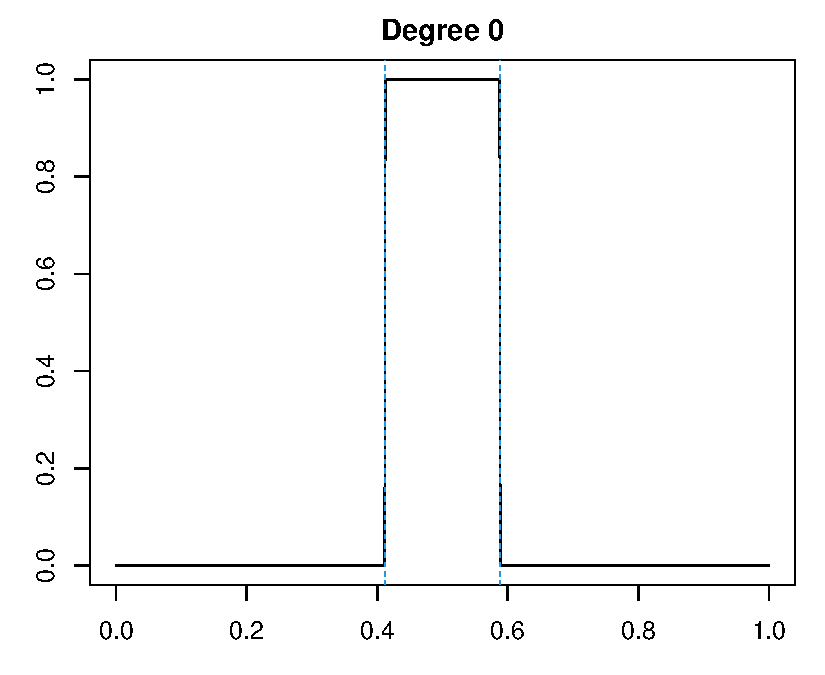
\includegraphics[width=0.475\textwidth]{bs0.pdf} 
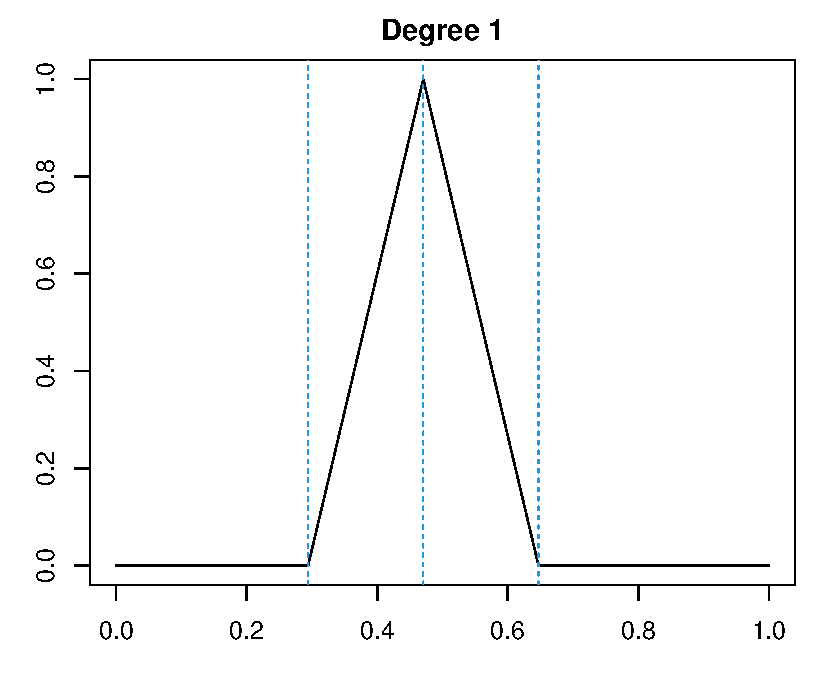
\includegraphics[width=0.475\textwidth]{bs1.pdf} 
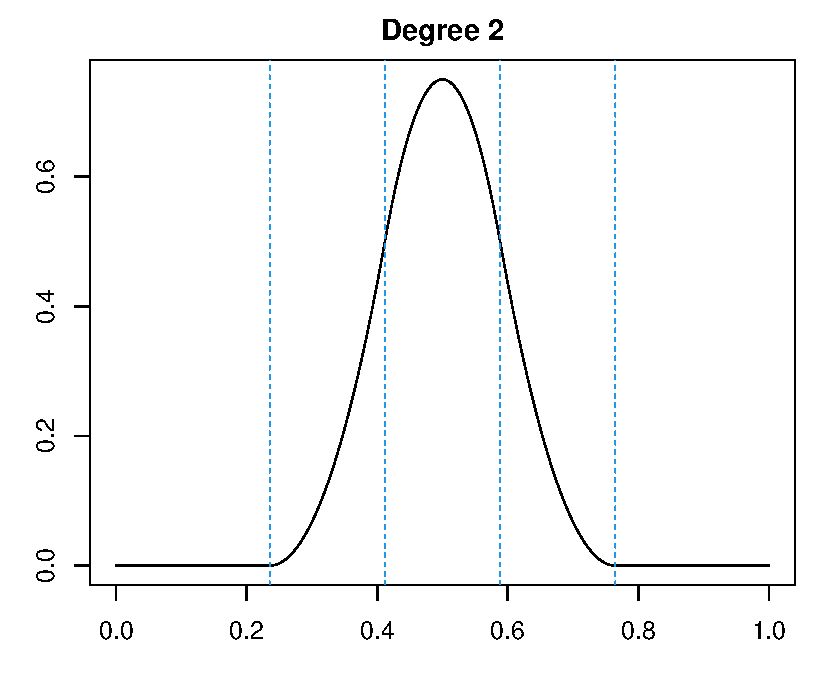
\includegraphics[width=0.475\textwidth]{bs2.pdf} 
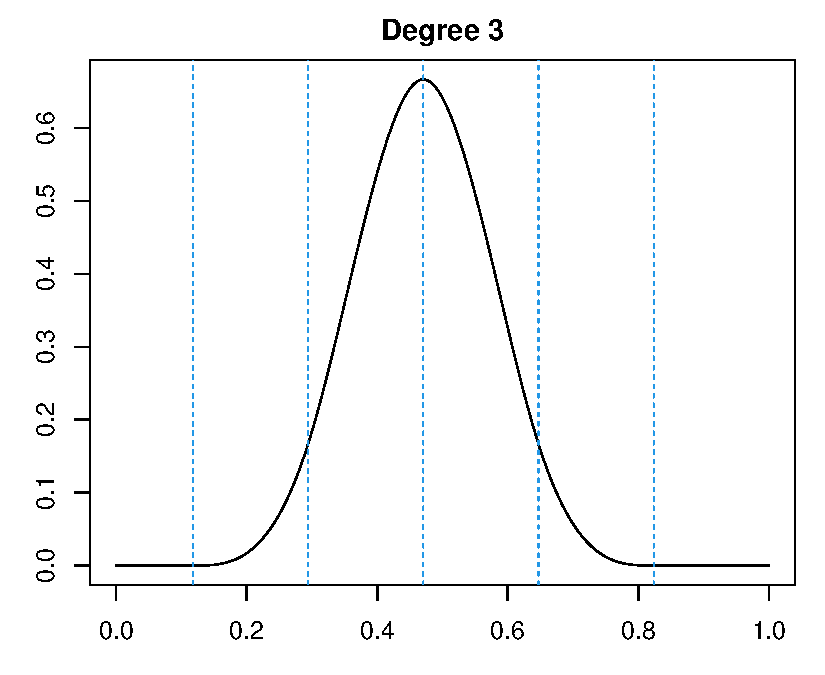
\includegraphics[width=0.475\textwidth]{bs3.pdf} 
\caption{\it B-splines of degrees 0 through 3. The knot points are marked by
  dashed blue vertical lines.}
\label{fig:bs}
\end{figure}

\paragraph{Recursive formulation.} 

B-splines satisfy a recursion relation that can be seen directly from the
recursive nature of divided differences: for any $k \geq 1$ and centers $z_1 <
\cdots < z_{k+2}$,  
\begin{align*}
(x - \cdot)^k_+ [z_1,\dots,z_{k+2}]
&= \frac{(x - \cdot)^k_+[z_2,\dots,z_{k+2}] - 
(x -\cdot)^k_+[z_1,\dots,z_{k+1}]}{z_{k+2} - z_1} \\
&= \frac{(x-z_{k+2})(x - \cdot)^{k-1}_+[z_2,\dots,z_{k+2}] 
- (x-z_1) (x - \cdot)^{k-1}_+[z_1,\dots,z_{k+1}] }{z_{k+2} - z_1},  
\end{align*} 
where in the second line we applied the Leibniz rule for divided differences 
\[
fg [z_1,\dots,z_{k+1}] = \sum_{i=1}^{k+1} f[z_1,\dots,z_i] g[z_i,\dots,z_{k+1}] 
\]
to conclude that
\begin{align*}
(x - \cdot)^k_+ [z_1,\dots,z_{k+1}] &= (x-z_1) \cdot 
(x - \cdot)^{k-1}_+ [z_1,\dots,z_{k+1}] \\
(x - \cdot)^k_+ [z_2,\dots,z_{k+2}] &= (x - \cdot)^{k-1}_+ 
  [z_2,\dots,z_{k+2}] \cdot (x-z_{k+2}). 
\end{align*}
Translating the above recursion over to normalized B-splines, we get 
\[
M^k(x; z_{1:(k+2)}) = \frac{x-z_1}{z_{k+1}-z_1} \cdot 
M^{k-1}(x; z_{1:(k+1)}) + \frac{z_{k+2}-x}{z_{k+2}-z_2} \cdot 
M^{k-1}(x; z_{2:(k+2)}),  
\]
which means that for the normalized basis, 
\[
M^k_j(x) = \frac{x-t_{j-k-1}}{t_{j-1}-t_{j-k-1}} \cdot
M^{k-1}_{j-1}(x) + \frac{t_j-x}{t_j-t_{j-k}} \cdot M^{k-1}_j(x), 
\quad j=1,\dots,r+k+1.  
\]
Above, we naturally interpret \smash{$M^{k-1}_0 = M^{k-1}(\cdot; 
  t_{-k:0})|_{[a,b]}$} and \smash{$M^{k-1}_{r+k+1} = M^{k-1}(\cdot;   
  t_{(r+1):(r+k+1)})|_{[a,b]}$}. 

The above recursions are very important, both for verifying numerous properties
of B-splines and for computational purposes. In fact, many authors prefer to
use recursion to define a B-spline basis in the first place.

\end{document}

